\iffalse
\let\negmedspace\undefined
\let\negthickspace\undefined
\documentclass[journal,12pt,twocolumn]{IEEEtran}
\usepackage{cite}
\usepackage{amsmath,amssymb,amsfonts,amsthm}
\usepackage{algorithmic}
\usepackage{graphicx}
\usepackage{textcomp}
\usepackage{xcolor}
\usepackage{txfonts}
\usepackage{listings}
\usepackage{enumitem}
\usepackage{mathtools}
\usepackage{gensymb}
\usepackage{comment}
\usepackage[breaklinks=true]{hyperref}
\usepackage{tkz-euclide} 
\usepackage{listings}
\usepackage{gvv}                                        
\def\inputGnumericTable{}                                 
\usepackage[latin1]{inputenc}                                
\usepackage{color}                                            
\usepackage{array}                                            
\usepackage{longtable}                                       
\usepackage{calc}                                             
\usepackage{multirow}                                         
\usepackage{hhline}                                           
\usepackage{ifthen}                                           
\usepackage{lscape}
\usepackage{caption}
\newtheorem{theorem}{Theorem}[section]
\newtheorem{problem}{Problem}
\newtheorem{proposition}{Proposition}[section]
\newtheorem{lemma}{Lemma}[section]
\newtheorem{corollary}[theorem]{Corollary}
\newtheorem{example}{Example}[section]
\newtheorem{definition}[problem]{Definition}
\newcommand{\BEQA}{\begin{eqnarray}}
\newcommand{\EEQA}{\end{eqnarray}}
\newcommand{\define}{\stackrel{\triangle}{=}}
\theoremstyle{remark}
\newtheorem{rem}{Remark}
\begin{document}

\bibliographystyle{IEEEtran}
\vspace{3cm}

\title{10.5.2.14}
\author{EE23BTECH11003 - pranav}
\maketitle
\newpage

\bigskip
\renewcommand{\thefigure}{\arabic{figure}}
\renewcommand{\thetable}{\arabic{table}}

\textbf{Question}:
How many multiples of 4 lie between 10 and 250?\\
\solution
\fi
\begin{table}[h]
    \centering
    \input{ncert-maths/10/5/2/14/tables/Table.Tex}
    \caption{Variables Used}
    \label{tab:10.5.2.14}
\end{table}
\begin{align}
    n&=\frac{(250-250 \text{ mod } 2)-(10+10\text{ mod } 2)}{4}+1\\
    n&=60
\end{align}
Considering the series to start from $n=0$,the general term is
\begin{align}
x(n)&=(x(0)+nd)u(n)\\
x(n)&=(12+4n)u(n)
\end{align}
\begin{figure}[h!]
    \centering
    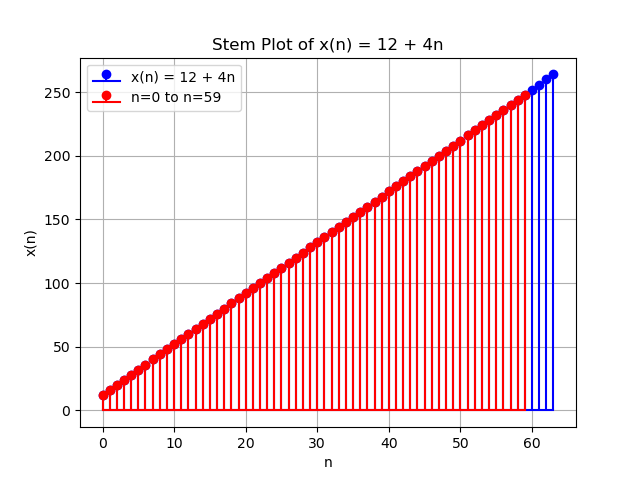
\includegraphics[width=\linewidth]{ncert-maths/10/5/2/14/figs/graph1.png}
    \caption{stem plot of x(n)}
\end{figure}
applying Z transform
\begin{align}
    X(z)&= \sum_{n=-\infty}^{\infty}x(n) z^{-n}\\
   \implies X(z)&= \sum_{n=-\infty}^{\infty} (12+4n) u(n) z^{-n}\\
   \implies X(z) &=\sum_{n= 0}^{\infty} (12+4n)  z^{-n}\\
   \implies X(z)&=\frac{12}{1-z^{-1}}+\frac{4 z^{-1}}{(1-z^{-1})^{2}}\quad \abs{z}>1
\end{align}
%\end{document}
